\documentclass[a4paper,onecolumn]{article}
\usepackage[page,toc,titletoc,title]{appendix}
\usepackage{url}
\usepackage{caption}
\usepackage{subcaption}
\usepackage{graphicx}
\usepackage[sc]{mathpazo} % Use the Palatino font
\usepackage[T1]{fontenc} % Use 8-bit encoding that has 256 glyphs
\usepackage[utf8]{inputenc} % Use utf-8 as encoding
\linespread{1.05} % Line spacing - Palatino needs more space between lines
\usepackage{microtype} % Slightly tweak font spacing for aesthetics
\usepackage[spanish, activeacute]{babel}
 \decimalpoint
% \usepackage[hmarginratio=1:1,top=32mm,columnsep=20pt]{geometry} % Document marginshttps://www.overleaf.com/project/60211b96f72a79d4c7515e93
% \usepackage[hang, small,labelfont=bf,up,textfont=it,up]{caption} % Custom captions under/above floats in tables or figures
\usepackage{verbatim} % comentarios
\usepackage{listings}
\usepackage{xcolor}
\usepackage{float}
\usepackage{adjustbox}
\lstset{
    inputencoding=utf8,
    language=SQL,
    frame=single,
    basicstyle=\ttfamily\small,
    keywordstyle=\color{blue}\bfseries,
    identifierstyle=\color{black},
    commentstyle=\color{gray}\itshape,
    stringstyle=\color{red},
    numbers=left,
    numberstyle=\tiny\color{gray},
    stepnumber=1,
    numbersep=10pt,
    showspaces=false,
    showstringspaces=false,
    breaklines=true,
    breakindent=0pt,
    breakatwhitespace=false,
    tabsize=2,
    captionpos=b
}
\setlength{\parskip}{0.8em}
\usepackage{natbib}
\usepackage{enumitem}
% \setlist[itemize]{noitemsep} % Make itemize lists more compact
% \usepackage{abstract} % Allows abstract customization
% \renewcommand{\abstractnamefont}{\normalfont\bfseries} % Set the "Abstract" text to bold
% \renewcommand{\abstracttextfont}{\normalfont\small\itshape} % Set the abstract itself to small italic text
\usepackage{titlesec}

\usepackage{fancyhdr} % Headers and footers
\pagestyle{fancy} % All pages have headers and footers
\fancyhead{}
\lhead{Hugo Gómez Sabucedo}
\rhead{Bases de datos SQL}

\renewcommand{\footrulewidth}{0.2pt}
\usepackage{titling} % Customizing the title section
\usepackage[breaklinks=true]{hyperref} % For hyperlinks in the PDF
%\usepackage{array}
%\newcolumntype{C}[1]{>{\centering\let\newline\\\arraybackslash\hspace{0pt}}m{#1}}
%\usepackage{lipsum} % NO NECESARIO LUEGO
%\usepackage{amsmath}
%\usepackage{wrapfig}
%\usepackage{multicol}
%\usepackage{bm}


\let\stdsection\section
\renewcommand\section{\newpage\stdsection}

%-------------------------------------------------------------------------------
%	TITLE SECTION
%-------------------------------------------------------------------------------

\setlength{\droptitle}{-4\baselineskip} % Move the title up



\title{\begin{center} \Huge Bases de datos NoSQL \end{center}} % Article title
\author{
    \textsc{\Huge Hugo Gómez Sabucedo} \\ % Your name
    \large \href{mailto:hugogomezsabucedo@gmail.com}{hugogomezsabucedo@gmail.com} \\ [2ex] % Your email address
    \Large \textbf{Máster Big Data, Data Science \& Inteligencia Artificial} \\
    \normalsize Curso 2024-2025 \\
    \large Universidad Complutense de Madrid
}
\date{} % Leave empty to omit a date

\begin{document}
% Print the title
\maketitle
%tableofcontents
\begin{sloppypar}

%-------------------------------------------------------------------------
%	DOCUMENT
%-------------------------------------------------------------------------

\section{Ejercicios} \label{ejericios}
A continuación se incluyen las capturas con las querys y los resultados de las ejecuciones de las consultas de los diferentes ejercicios, así como una breve 
explicación de las mismas (si es necesario). He incluido también el archivo \texttt{JavaScript} con todas las consultas al final del archivo y como adjunto.

\begin{enumerate} \setcounter{enumi}{-1}
    \item \textbf{Importación del fichero en una colección llamada movies}: se ha creado la colección movies dentro de la base de datos \textit{clases} e
    importado los datos usando la funcionalidad ''Add data'' de MongoDBCompass, importando los datos directamente desde el archivo JSON.
    \begin{center}
        \begin{figure}[h!]
            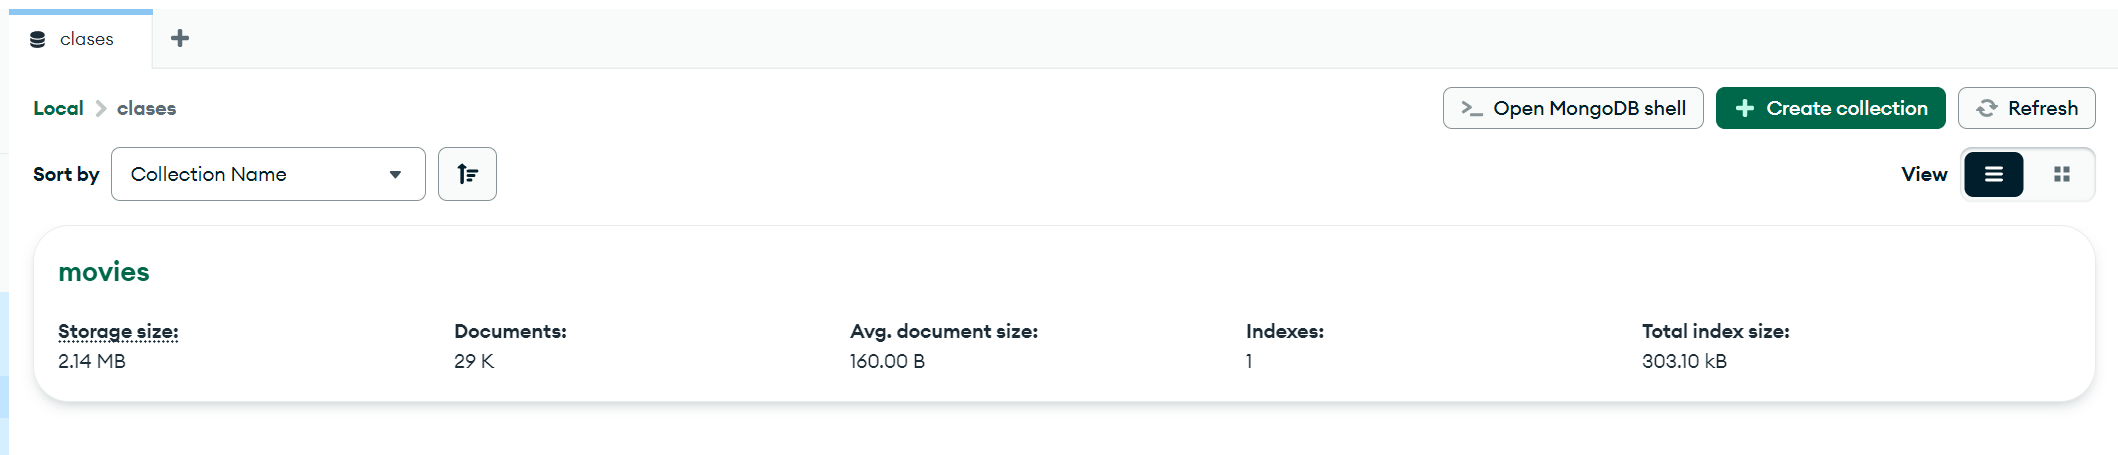
\includegraphics[width=\textwidth]{querys/0.png}
        \end{figure}
    \end{center}
    \item \textbf{Analizar con find la colección}.
    \begin{center}
        \begin{figure}[h!]
            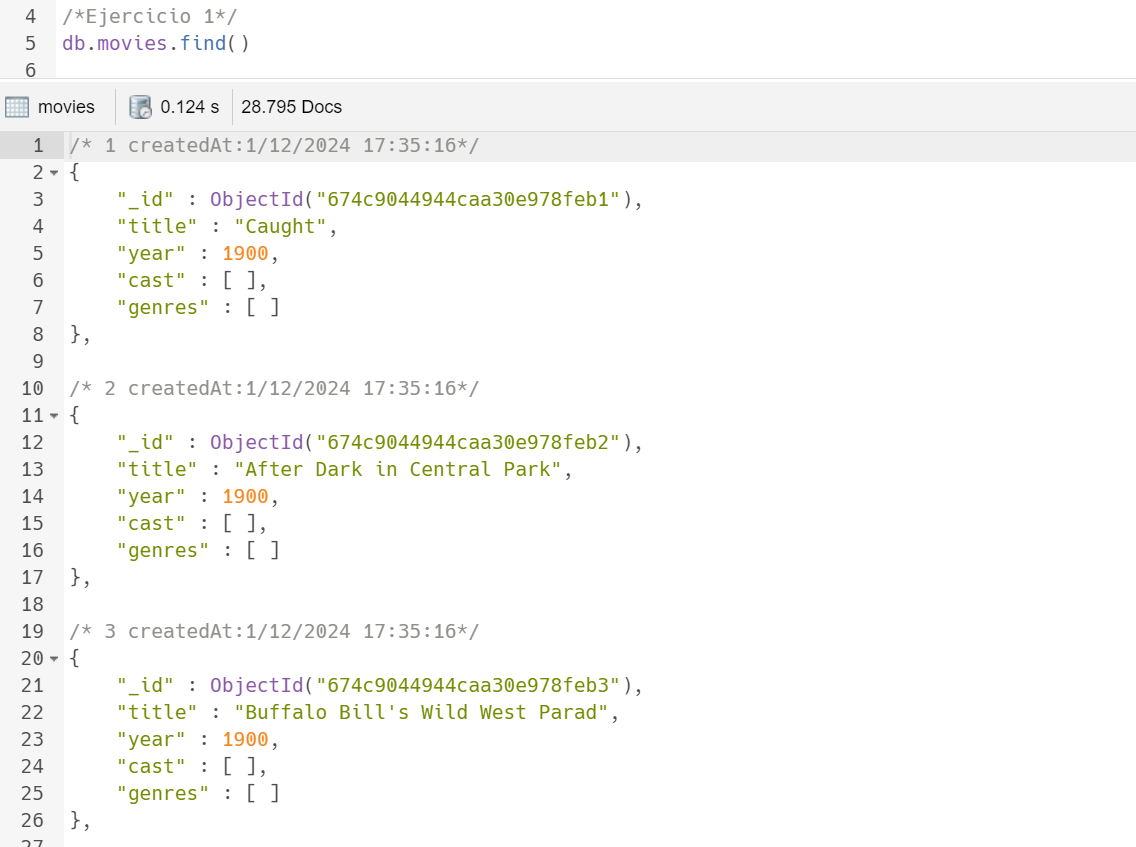
\includegraphics[width=\textwidth]{querys/1.png}
        \end{figure}
    \end{center}
    \item \textbf{Contar cuantos documentos (películas) tiene cargado}.
    \begin{center}
        \begin{figure}[H]
            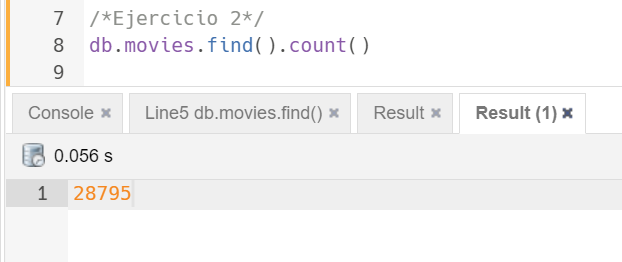
\includegraphics[width=\textwidth]{querys/2.png}
        \end{figure}
    \end{center}
    \item \textbf{Insertar una película}. Se crea una película \textit{test} para insertar.
    \begin{center}
        \begin{figure}[h!]
            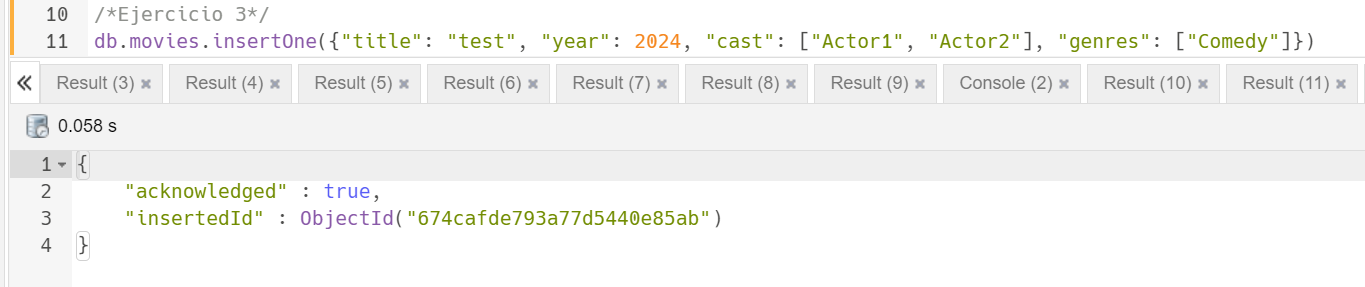
\includegraphics[width=\textwidth]{querys/3.png}
        \end{figure}
    \end{center}
    \item \textbf{Borrar la película insertada en el punto anterior}. Como la película se llama \textit{text} y es del año 2024 (más adelante se comprobará
    que no hay ninguna película de este año), se borra en base a esto. Borrar en base al id no es efectivo, ya que si se reejecuta la query este cambiará.
    \begin{center}
        \begin{figure}[h!]
            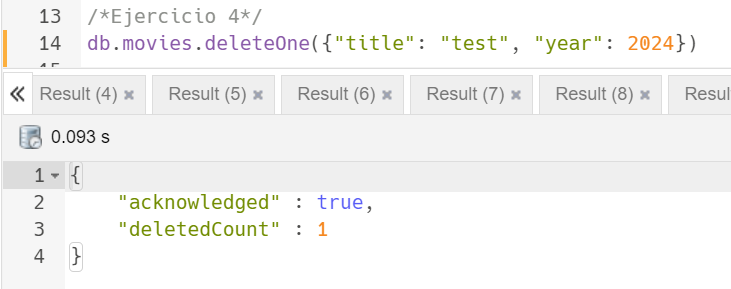
\includegraphics[width=\textwidth]{querys/4.png}
        \end{figure}
    \end{center}
    \item \textbf{Contar cuantas películas tienen actores que se llaman ''and''}.
    \begin{center}
        \begin{figure}[H]
            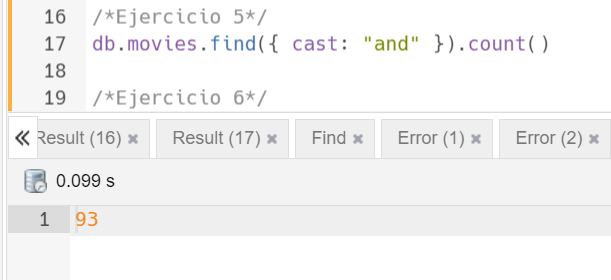
\includegraphics[width=\textwidth]{querys/5.png}
        \end{figure}
    \end{center}
    \item \textbf{Actualizar los documentos cuyo actor tenga el valor ''and'', sacando ese valor del array cast}. Usamos \texttt{updateMany} porque se actualizarán
    varios documentos a la vez. Se busca, como antes, las que tengan ''and'', y se eliminan estos del array con \texttt{\$pull}.
    \begin{center}
        \begin{figure}[h!]
            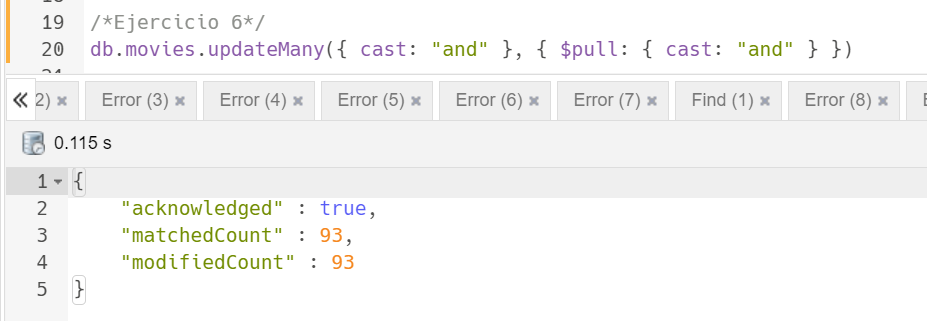
\includegraphics[width=\textwidth]{querys/6.png}
        \end{figure}
    \end{center}
\newpage
\item \textbf{Contar cuantos documentos tienen el array ''cast'' vacío}.
    \begin{center}
        \begin{figure}[h!]
            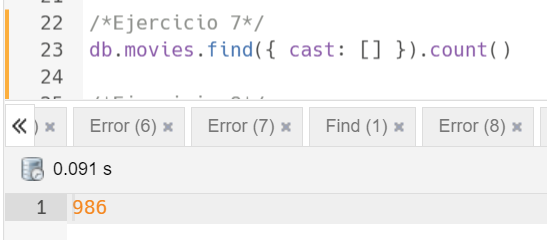
\includegraphics[width=\textwidth]{querys/7.png}
        \end{figure}
    \end{center}
    \item \textbf{Actualizar todos los documentos que tengan el array cast vacío, añadiendo un nuevo elemento con el valor Undefined}. Con el \texttt{updateMany},
    actualizamos el campo cast al array \textit{[''Undefined'']}, para asegurarnos que se sigue manteniendo el tipo del mismo.
    \begin{center}
        \begin{figure}[h!]
            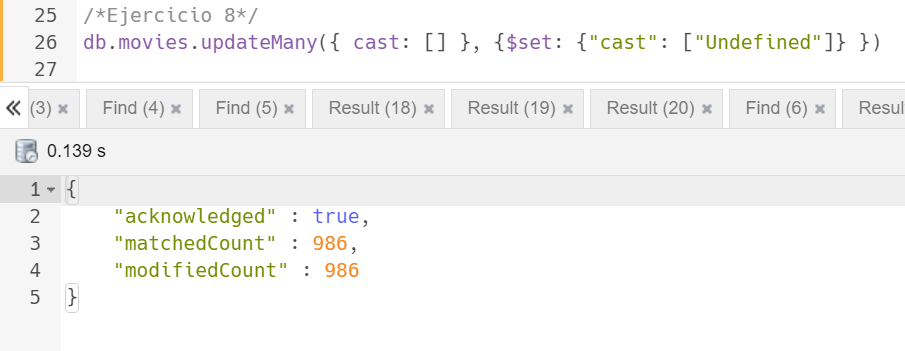
\includegraphics[width=\textwidth]{querys/8.png}
        \end{figure}
    \end{center}
    \item \textbf{Contar cuantos documentos tienen el array genres vacío}.
    \begin{center}
        \begin{figure}[H]
            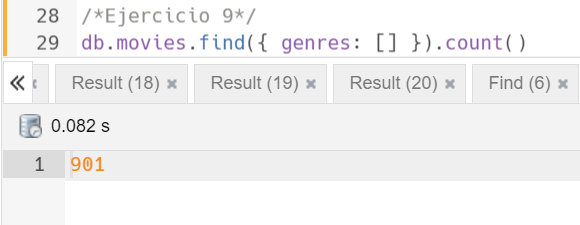
\includegraphics[width=\textwidth]{querys/9.png}
        \end{figure}
    \end{center}
    \item \textbf{Actualizar todos los documentos que tengan el array genres vacío, añadiendo un nuevo elemento con el valor Undefined}. Hacemos lo mismo que en el caso del cast.
    \begin{center}
        \begin{figure}[h!]
            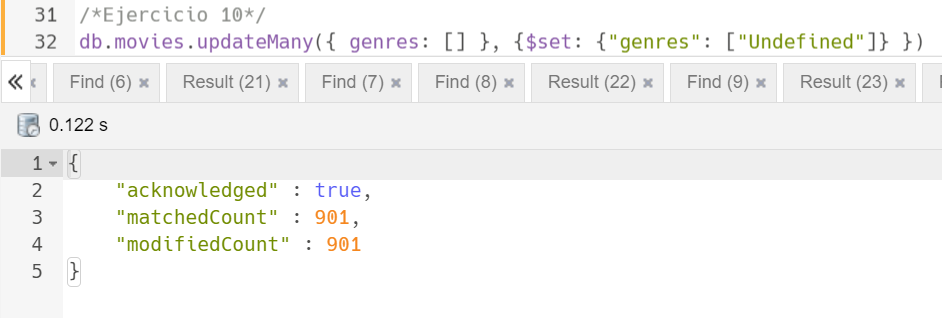
\includegraphics[width=\textwidth]{querys/10.png}
        \end{figure}
    \end{center}
    \item \textbf{Mostrar el año más reciente/actual que tenemos sobre todas las películas}. Buscamos solo los años, lo ordenamos de forma descendente y limitamos a 1 el output.
    \begin{center}
        \begin{figure}[h!]
            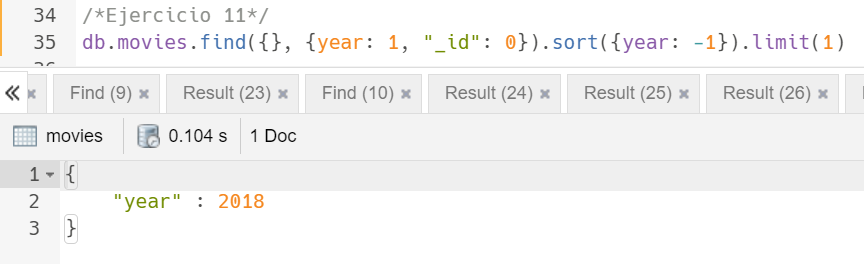
\includegraphics[width=\textwidth]{querys/11.png}
        \end{figure}
    \end{center}
    \newpage
    \item \textbf{Contar cuantas películas han salido en los últimos 20 años, desde el último año que se tienen películas en la colección}. Primero, buscamos el año más reciente. Luego, le restamos 20.
    Como las variables minYear y maxYear se definen fuera, las tenemos que pasar al pipeline usando \texttt{let}. A continuación hacemos un match y, como queremos comparar los campos del mismo documento,
    usamos el \texttt{\$expr}. Ya que restamos 20 al año para hallar el inicio del intervalo, debemos indicar que sea \textit{greater than} (para que no lo coja), mientras que para el fin debemos indicar \textit{less than or equal}.
    Con \texttt{\$size}, contamos el número de películas, y seleccionamos para el output el id y este total.
    \begin{center}
        \begin{figure}[h!]
            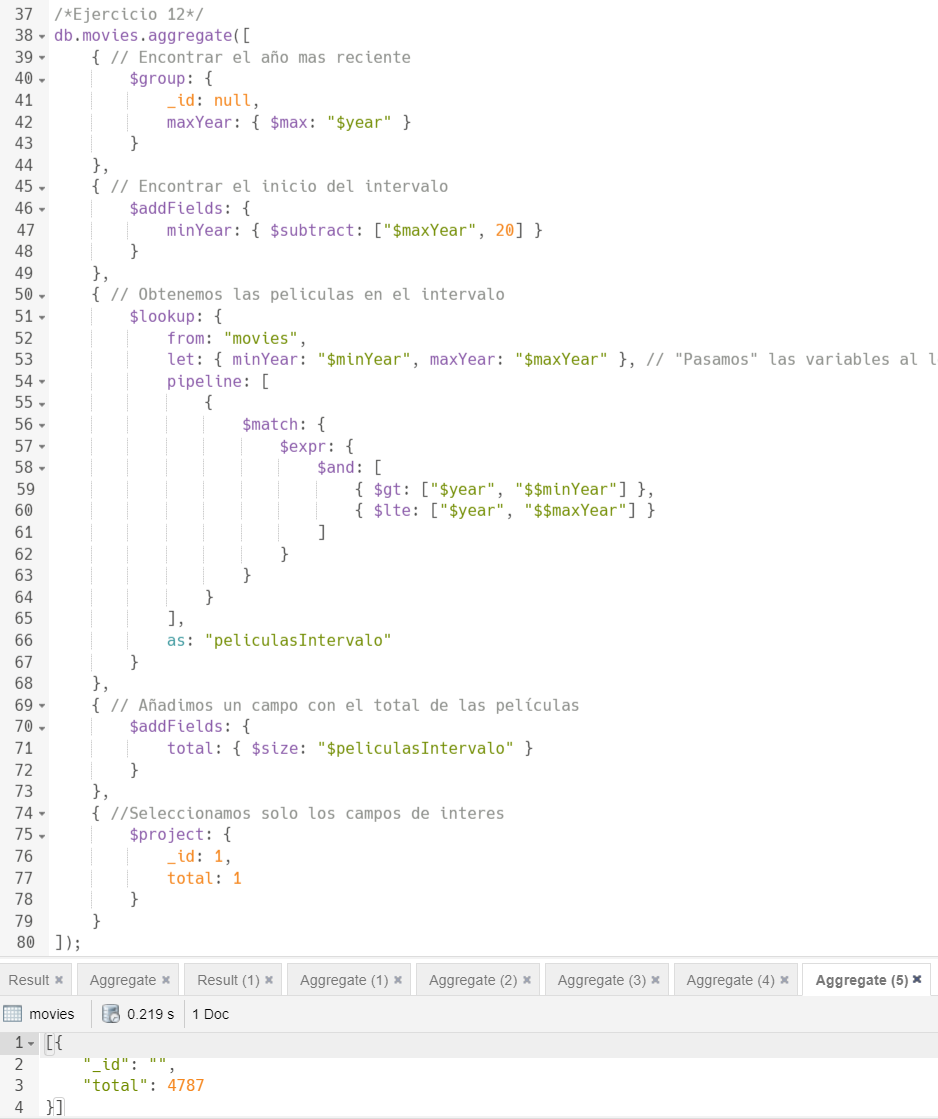
\includegraphics[width=\textwidth]{querys/12.png}
        \end{figure}
    \end{center}
    \newpage
    \item \textbf{Contar cuantas películas han salido en la década de los 60}. En este caso, como es un rango fijo, simplemente hacemos un \texttt{\$match}, incluyendo los años límite del intervalo, y calculamos el total como \texttt{\$sum: 1}
    (como 1 es siempre true, esta es una buena forma también de contar todos los documentos).
    \begin{center}
        \begin{figure}[h!]
            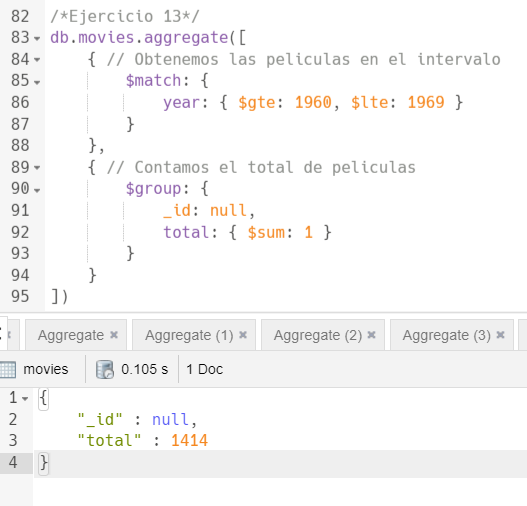
\includegraphics[width=\textwidth]{querys/13.png}
        \end{figure}
    \end{center}
    \newpage
    \item \textbf{Mostrar el año/años con más películas}. En primer lugar, agrupamos por año y contamos las películas de cada año.
    Luego, con otro \texttt{\$group}, encontramos el máximo número. Nos creamos un array con todos los años y el total de películas y, adicionalmente, el máximo.
    Separamos ''years'' en documentos individuales y, sobre esto, filtramos los que tengan el total igual al máximo, devolviendo los años como id y el total.
    Crear un array con los años y las películas nos sirve para manejar el caso en el que haya varios años con el máximo de películas, ya que se nos devolverían dichos años.
    \begin{center}
        \begin{figure}[H]
            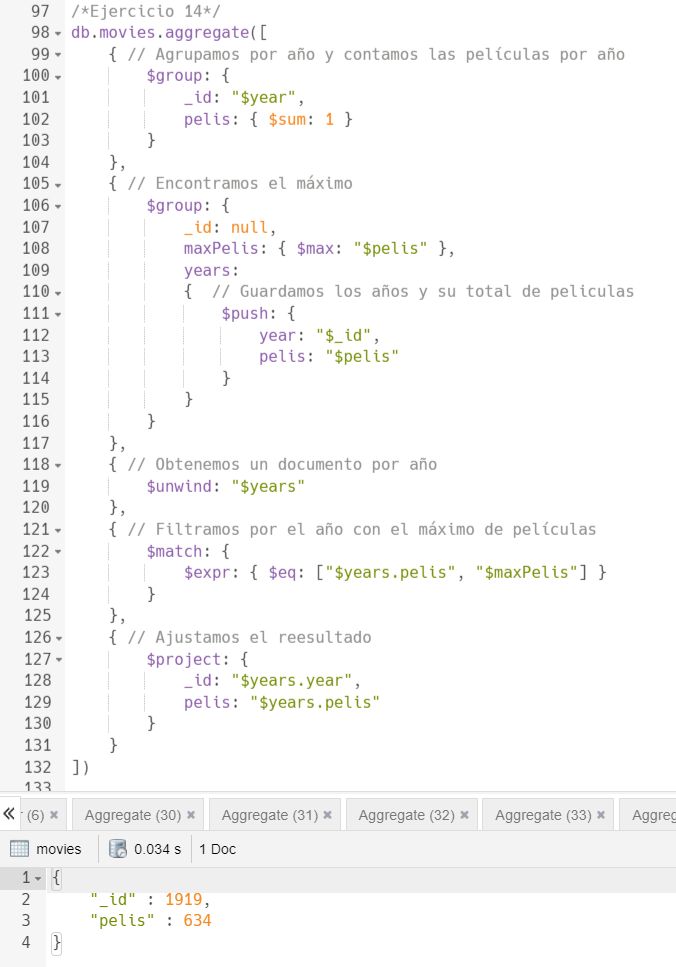
\includegraphics[width=0.9\textwidth]{querys/14.png}
        \end{figure}
    \end{center}
    \item \textbf{Mostrar el año/años con menos películas}. Procedemos igual que en el caso anterior, pero esta vez hallando el mínimo.
    \begin{center}
        \begin{figure}[h!]
            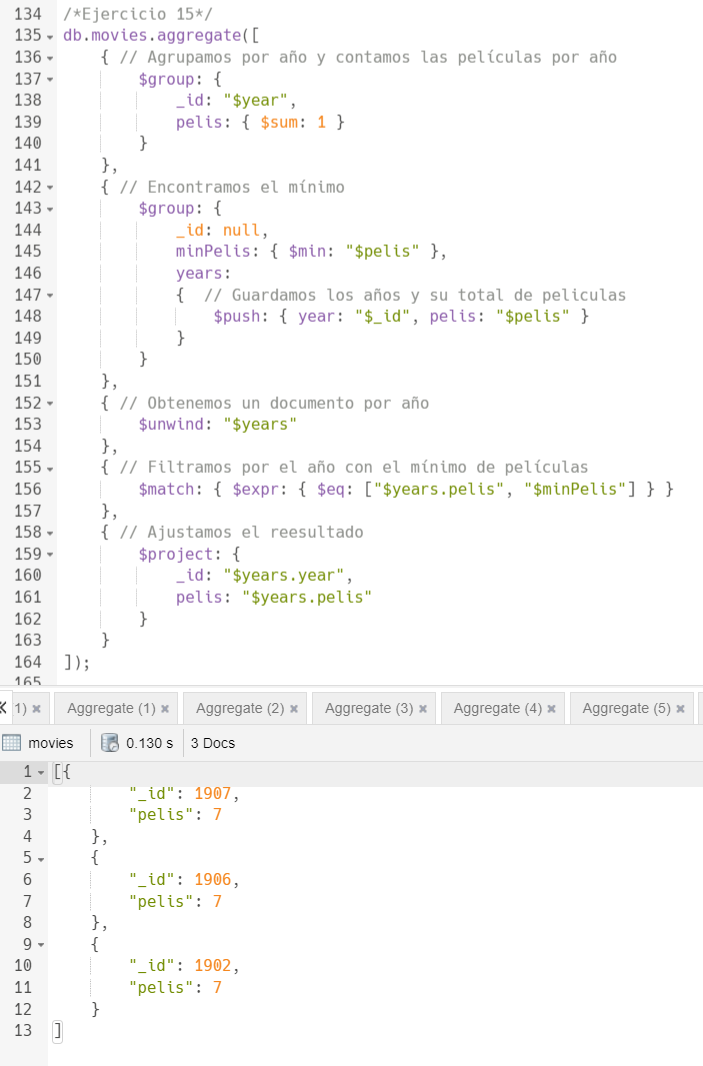
\includegraphics[width=\textwidth]{querys/15.png}
        \end{figure}
    \end{center}
    \item \textbf{Guardar en una nueva colección llamada ''actors'', haciendo \$unwind por actor. Contar cuantos elementos existen en la nueva colección}.
    Hacemos el unwind indicado, eliminamos el campo id (para que no este no se detecte como el campo id a usar por MongoDB y nos de error por tener IDs duplicados) y guardamos en la colección indicada.
    Luego se hace un count para contar el número de documentos que tiene la colección.
    \begin{center}
        \begin{figure}[h!]
            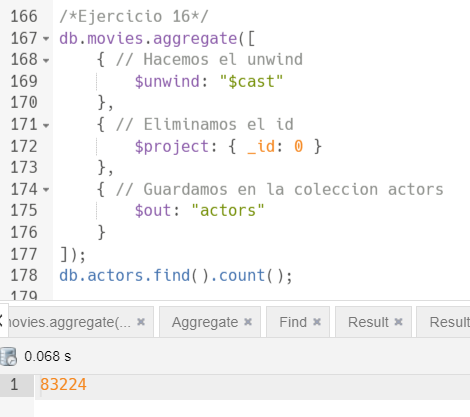
\includegraphics[width=\textwidth]{querys/16.png}
        \end{figure}
    \end{center}
    \newpage
    \item \textbf{Sobre \underline{actors}, mostrar la lista con los 5 actores que han participado en más películas, mostrando el número de películas en las que ha participado}.
    Primero excluimos los actores Undefined. Agrupamos por actor, contamos sus apariciones, ordenamos por este nuevo campo de forma descendente, y nos quedamos con los cinco primeros resultados.
    \begin{center}
        \begin{figure}[h!]
            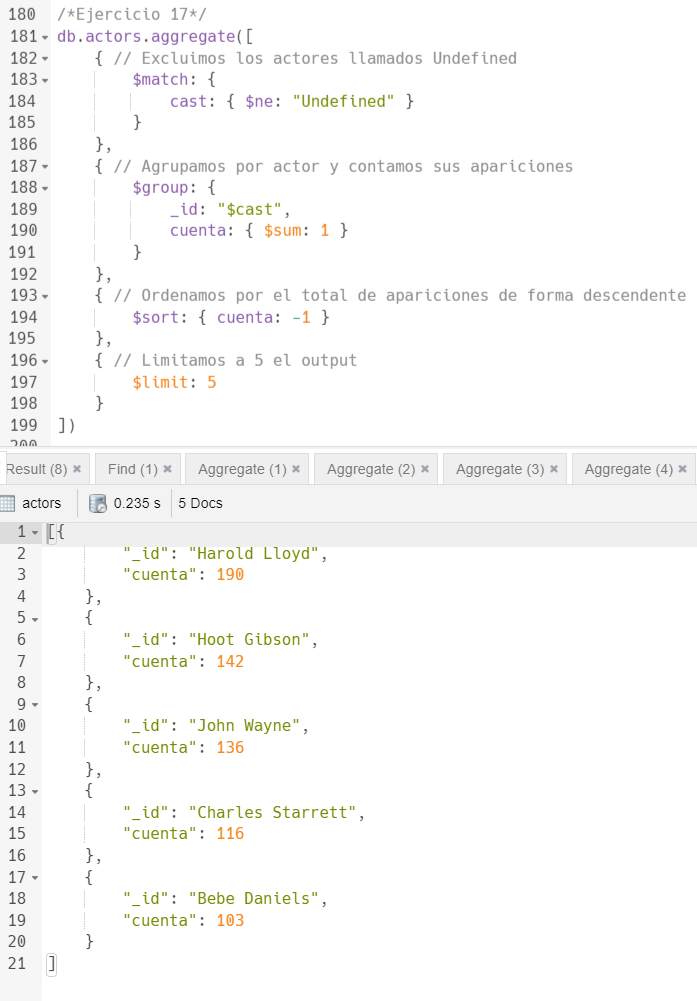
\includegraphics[width=\textwidth]{querys/17.png}
        \end{figure}
    \end{center}
    \item \textbf{Sobre \underline{actors}, agrupar por película y año, mostrando las 5 en las que más actores hayan participado, mostrando el número total de actores}.
    Realizamos la agrupación, contamos el total de actores, ordenamos por el total de forma descendente y nos quedamos con los cinco primeros.
    %\begin{center}
        \begin{figure}[h!]
            \begin{subfigure}[b]{0.5\textwidth}
                \centering
                \adjustbox{valign=m}{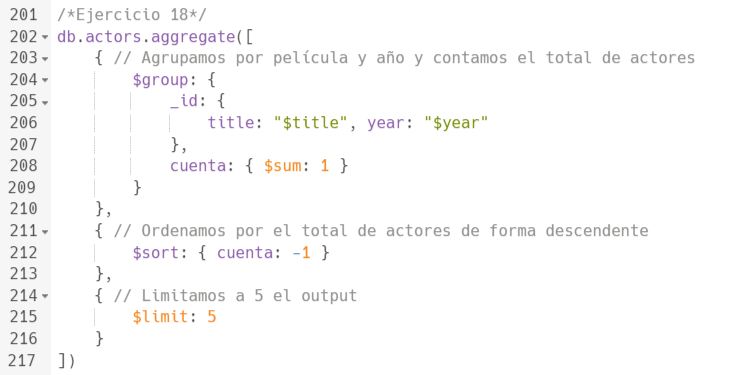
\includegraphics[width=\textwidth]{querys/18_query.png}}
            \end{subfigure}
            \hfill
            \begin{subfigure}[b]{0.5\textwidth}
                \adjustbox{valign=m}{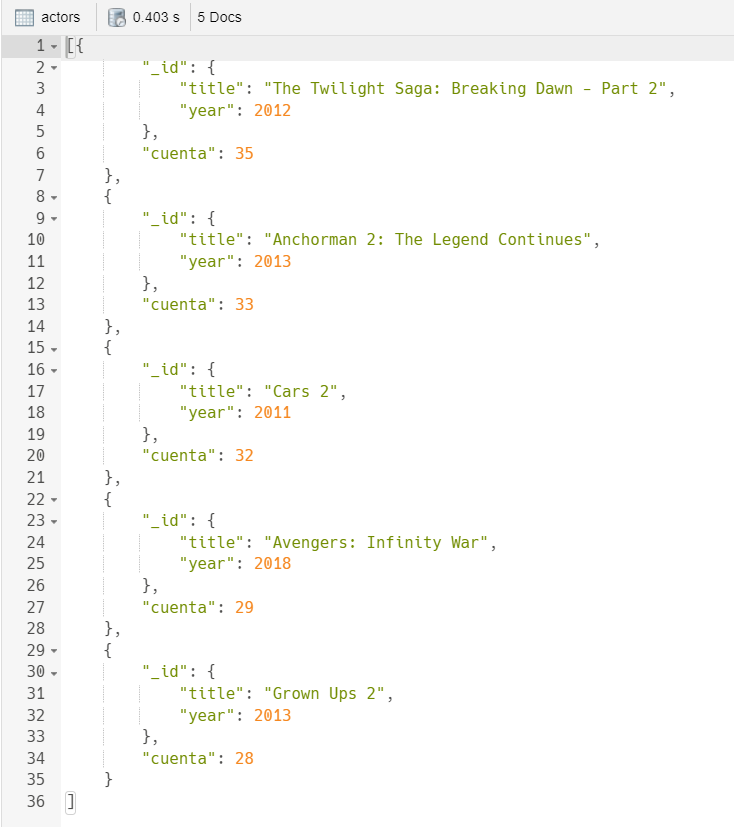
\includegraphics[width=\textwidth]{querys/18_result.png}}
            \end{subfigure}
       \end{figure}
    %\end{center}
    \newpage
    \item \textbf{Sobre \underline{actors}, mostrar los 5 actores cuya carrera haya sido la más larga, mostrando cuando comenzó, cuando finalizó y cuántos años ha trabajado}.
    Se agrupa por actor y se halla la fecha de inicio y de fin como el año mínimo y máximo. Se añade un campo con los años trabajados, haciendo un \texttt{\$subtract}.
    Se ordena por este campo y se limita a cinco el resultado.
    \begin{center}
        \begin{figure}[H]
            \centering
            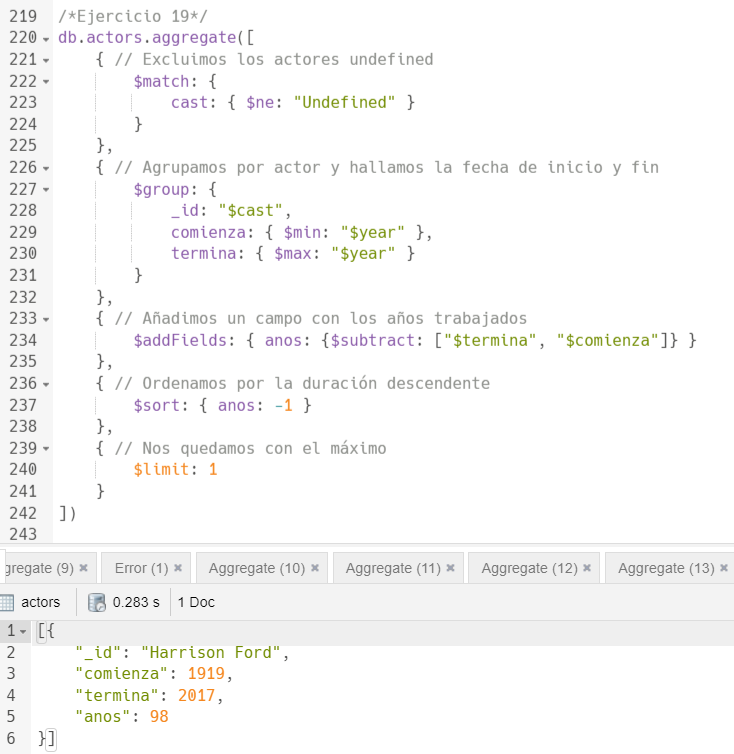
\includegraphics[width=\textwidth]{querys/19.png}
        \end{figure}
    \end{center}
    \newpage
    \item \textbf{Sobre \underline{actors}, guardar en una nueva colección llamada ''genres'' realizando la fase \$unwind por genres. Contar cuantos elementos existen en al nueva colección}.
    Hacemos el unwind indicado, eliminamos el campo id y guardamos en la colección.
    \begin{center}
        \begin{figure}[h!]
            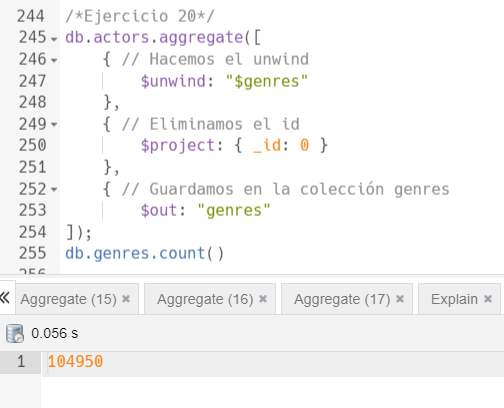
\includegraphics[width=0.75\textwidth]{querys/20.png}
        \end{figure}
    \end{center}
    \newpage
    \item \textbf{Sobre \underline{genres}, mostrar los 5 documentos agrupados por Año y Género que más número de películas diferentes tienen, mostrando el total de películas}.
    Agrupamos por año y por género, y usamos el \texttt{\$addToSet} para hallar las películas únicas (ya que un set se compone de elementos únicos, sin duplicados). Sobre este set,
    contamos las películas, ordenamos de forma descendente y limitamos a 5 el output.
    \begin{figure}[H]
        \begin{subfigure}[b]{0.6\textwidth}
            \centering
            \adjustbox{valign=m}{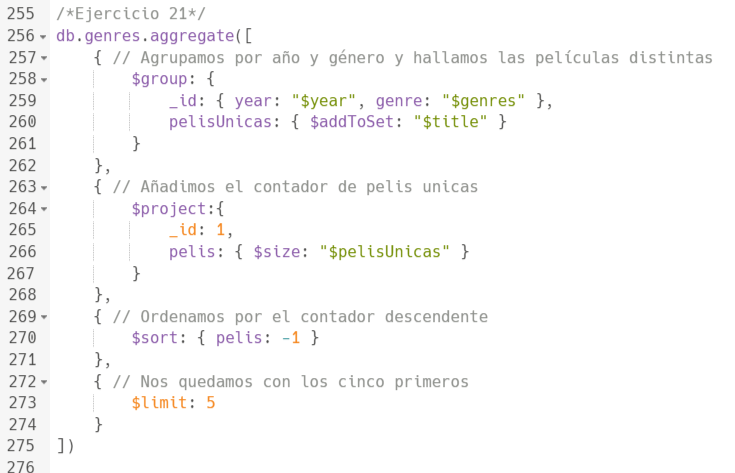
\includegraphics[width=\textwidth]{querys/21_query.png}}
        \end{subfigure}
        \hfill
        \begin{subfigure}[b]{0.4\textwidth}
            \adjustbox{valign=m}{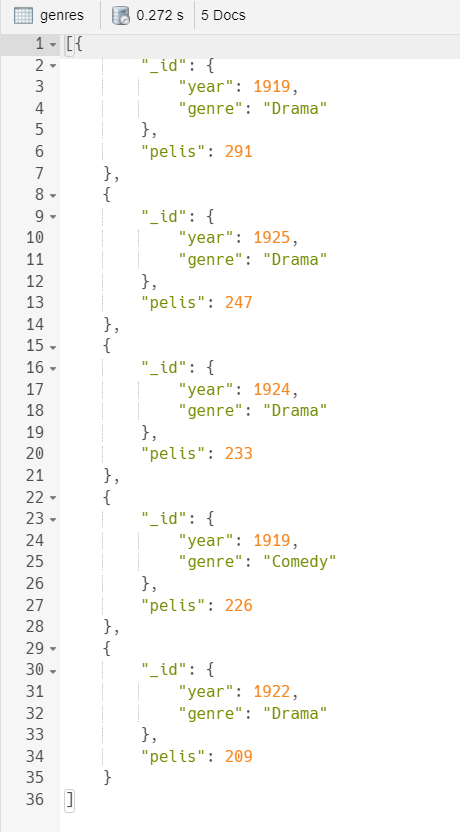
\includegraphics[width=\textwidth]{querys/21_result.png}}
        \end{subfigure}
   \end{figure}
   \newpage
    \item \textbf{Sobre \underline{genres}, mostrar los 5 actores y lo géneros en los que han participado con más número de géneros diferentes, mostrando el número de géneros}.
    Se agrupa por actor y, como antes, se añaden los géneros a un set. Se cuentan, se ordena y se limita a 5 el output.
    \begin{figure}[H]
        \begin{subfigure}[b]{.6\textwidth}
            \centering
            \adjustbox{valign=m}{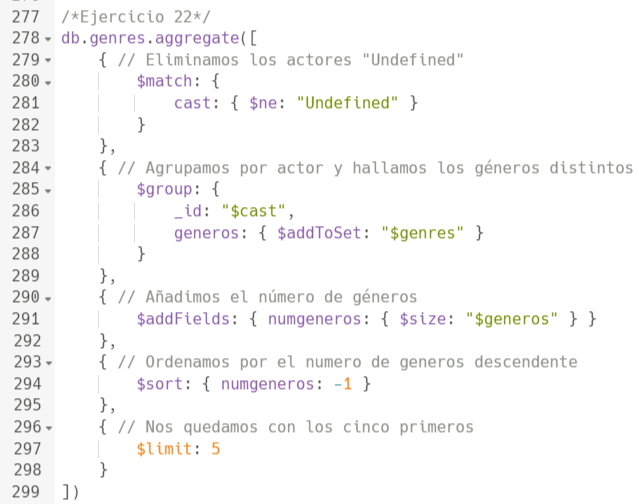
\includegraphics[width=\textwidth]{querys/22_query.png}}
        \end{subfigure}
        \vskip\baselineskip
        \begin{subfigure}[b]{0.34\textwidth}
            \adjustbox{valign=m}{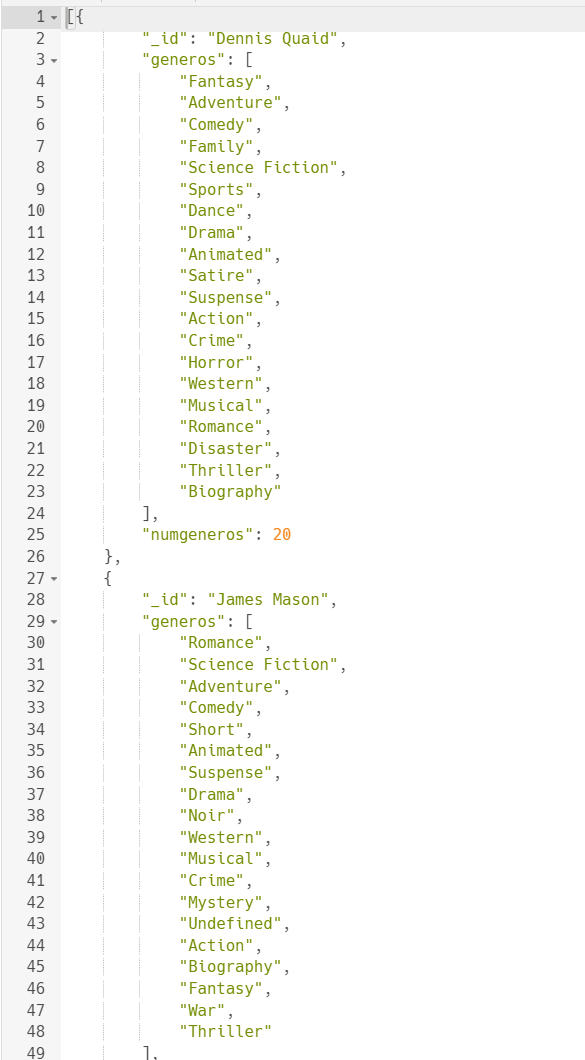
\includegraphics[width=\textwidth]{querys/22_result1.png}}
        \end{subfigure}
        %\hfill
        \begin{subfigure}[b]{0.34\textwidth}
            \centering
            \adjustbox{valign=m}{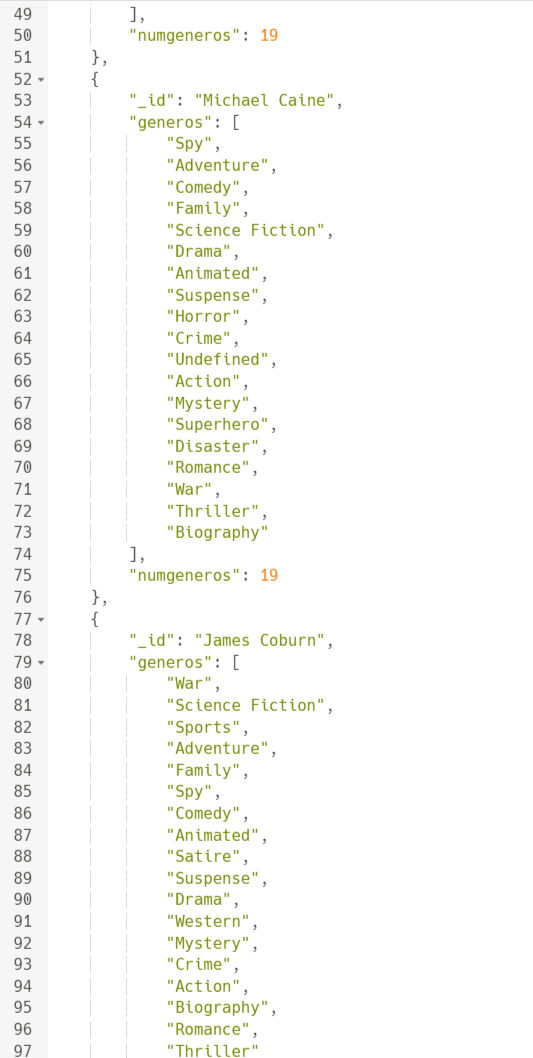
\includegraphics[width=\textwidth]{querys/22_result2.png}}
        \end{subfigure}
        %\hfill
        \begin{subfigure}[b]{0.3\textwidth}
            \adjustbox{valign=m}{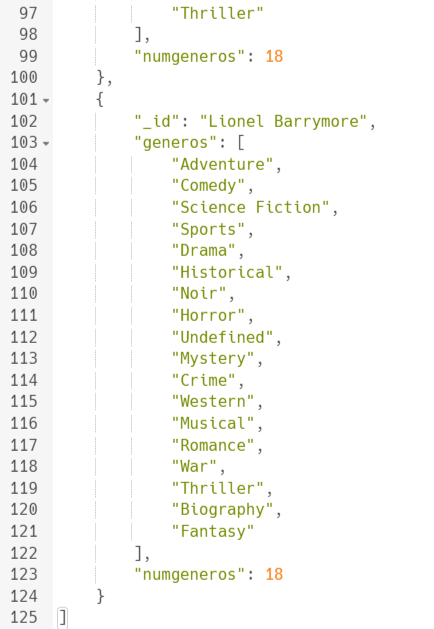
\includegraphics[width=\textwidth]{querys/22_result3.png}}
        \end{subfigure}
   \end{figure}
   \newpage
    \item \textbf{Sobre \underline{genres}, mostrar las 5 películas y su año, en los que más géneros diferentes han sido catalogados, mostrando esos géneros y el número}.
    Se agrupa por título y año y se hallan los géneros diferentes añadiendo a un set. Se cuenta, se ordena y se limita el output.
    \begin{figure}[H]
        \begin{subfigure}[b]{.6\textwidth}
            \centering
            \adjustbox{valign=m}{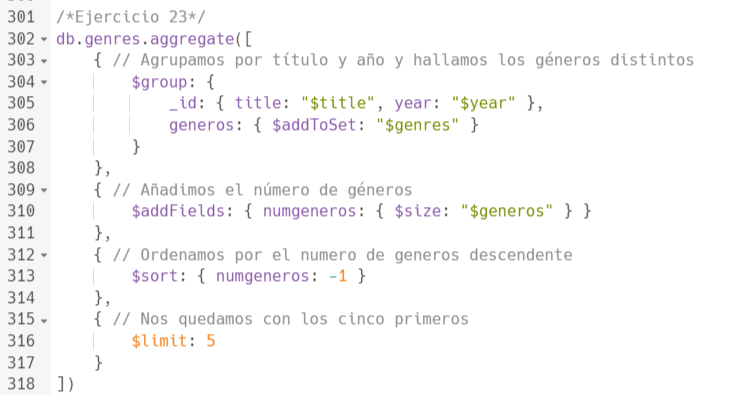
\includegraphics[width=\textwidth]{querys/23_query.png}}
        \end{subfigure}
        \vskip\baselineskip
        \begin{subfigure}[b]{0.45\textwidth}
            \centering
            \adjustbox{valign=m}{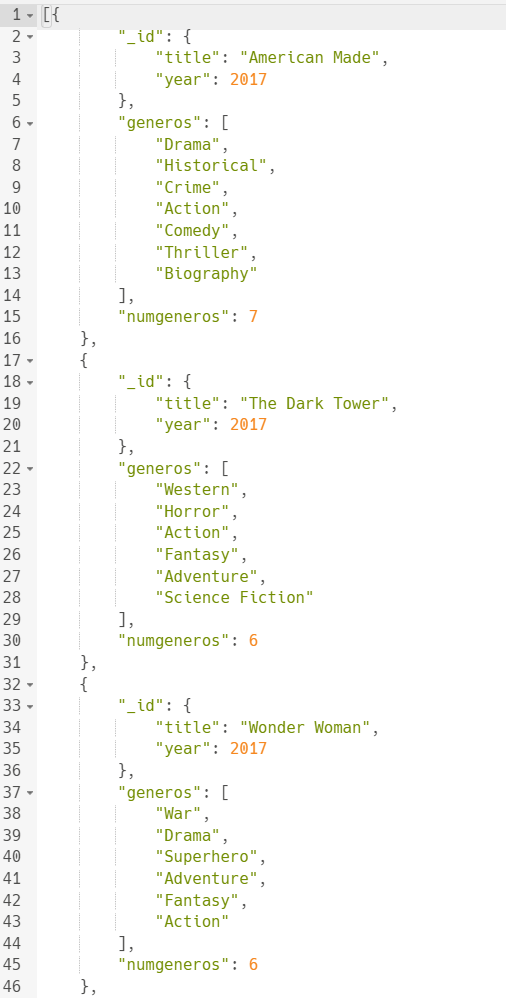
\includegraphics[width=\textwidth]{querys/23_result1.png}}
        \end{subfigure}
        \hfill
        \begin{subfigure}[b]{0.45\textwidth}
            \adjustbox{valign=m}{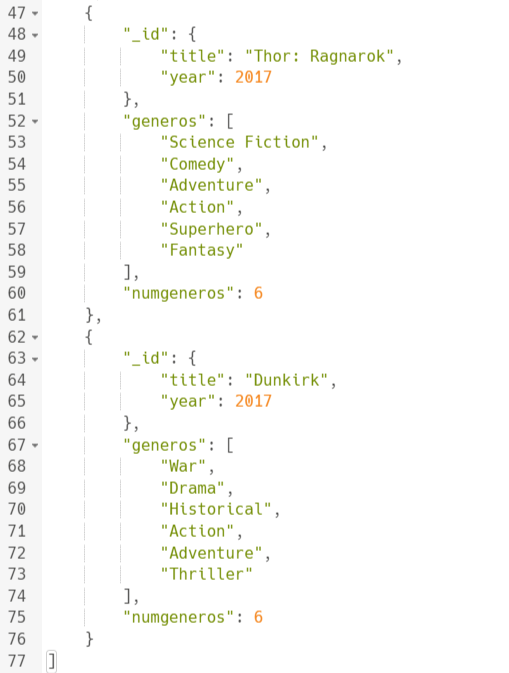
\includegraphics[width=\textwidth]{querys/23_result2.png}}
        \end{subfigure}
   \end{figure}
   \newpage
    \item \textbf{Ejercicio libre. Mostrar la películas con el reparto más grande, es decir, con el mayor número de actores. Mostrar la película, el año, los actores y el tamaño del cast}.
    Para este ejercicio, se añade un campo con el tamaño del cast, para ordenar de forma descendente, limitar a 1 el output y eliminar el id de la misma del output.
    \begin{figure}[H]
        \begin{subfigure}[b]{0.6\textwidth}
            \centering
            \adjustbox{valign=m}{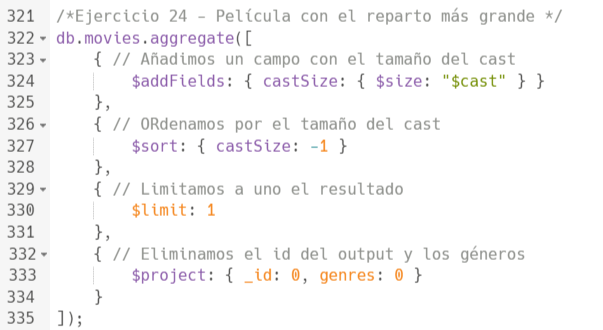
\includegraphics[width=\textwidth]{querys/24_query.png}}
        \end{subfigure}
        \hfill
        \begin{subfigure}[b]{0.4\textwidth}
            \adjustbox{valign=m}{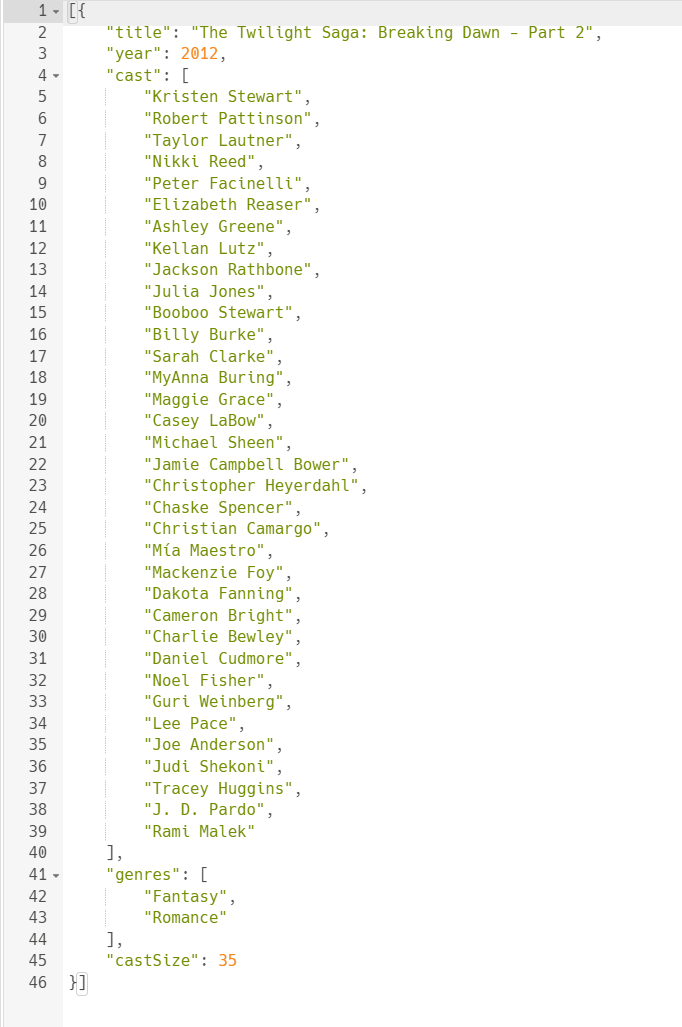
\includegraphics[width=\textwidth]{querys/24_result.png}}
        \end{subfigure}
   \end{figure}
    \item \textbf{Ejercicio libre. Sobre \underline{actors}, mostrar el actor más popular en cada género (es decir, el que más veces ha actuado)}. 
    Primero, excluimos los actores y géneros que sean Undefined. Se hace un unwind de los géneros, para desglosar; se agrupa por género y actor y se cuentan las películas.
    Se ordena por género, y por el total de películas (de forma descendente), y volvemos a agrupar por género, para obtener el primer actor, que se corresponderá con el actor más popular.
    Se seleccionan los campos de interés.
    \begin{figure}[H]
        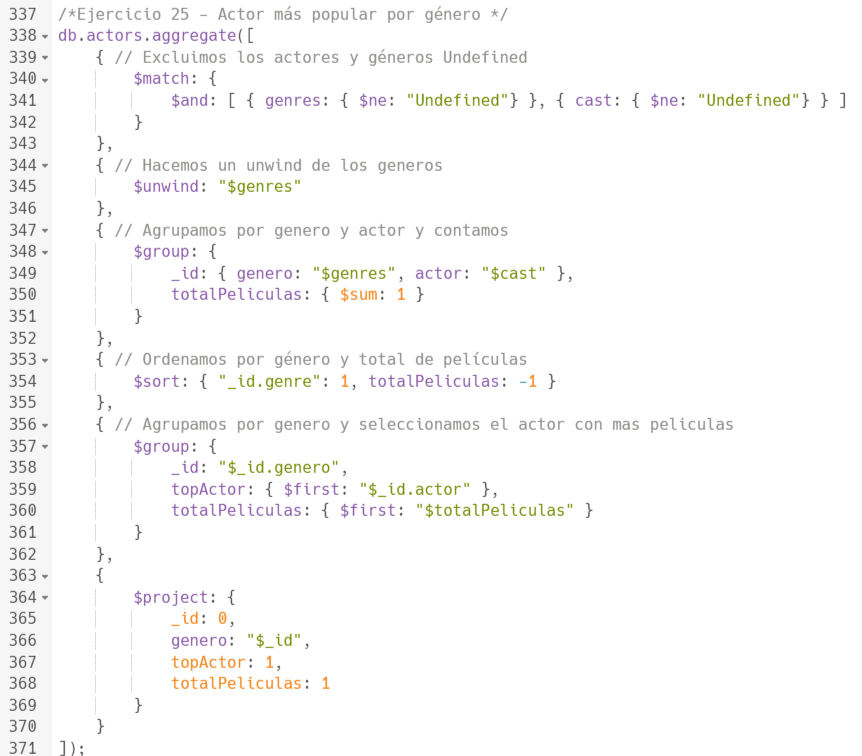
\includegraphics[width=0.6\linewidth]{querys/25_query.png}
    \end{figure}
    \begin{figure}[H]
            \centering
            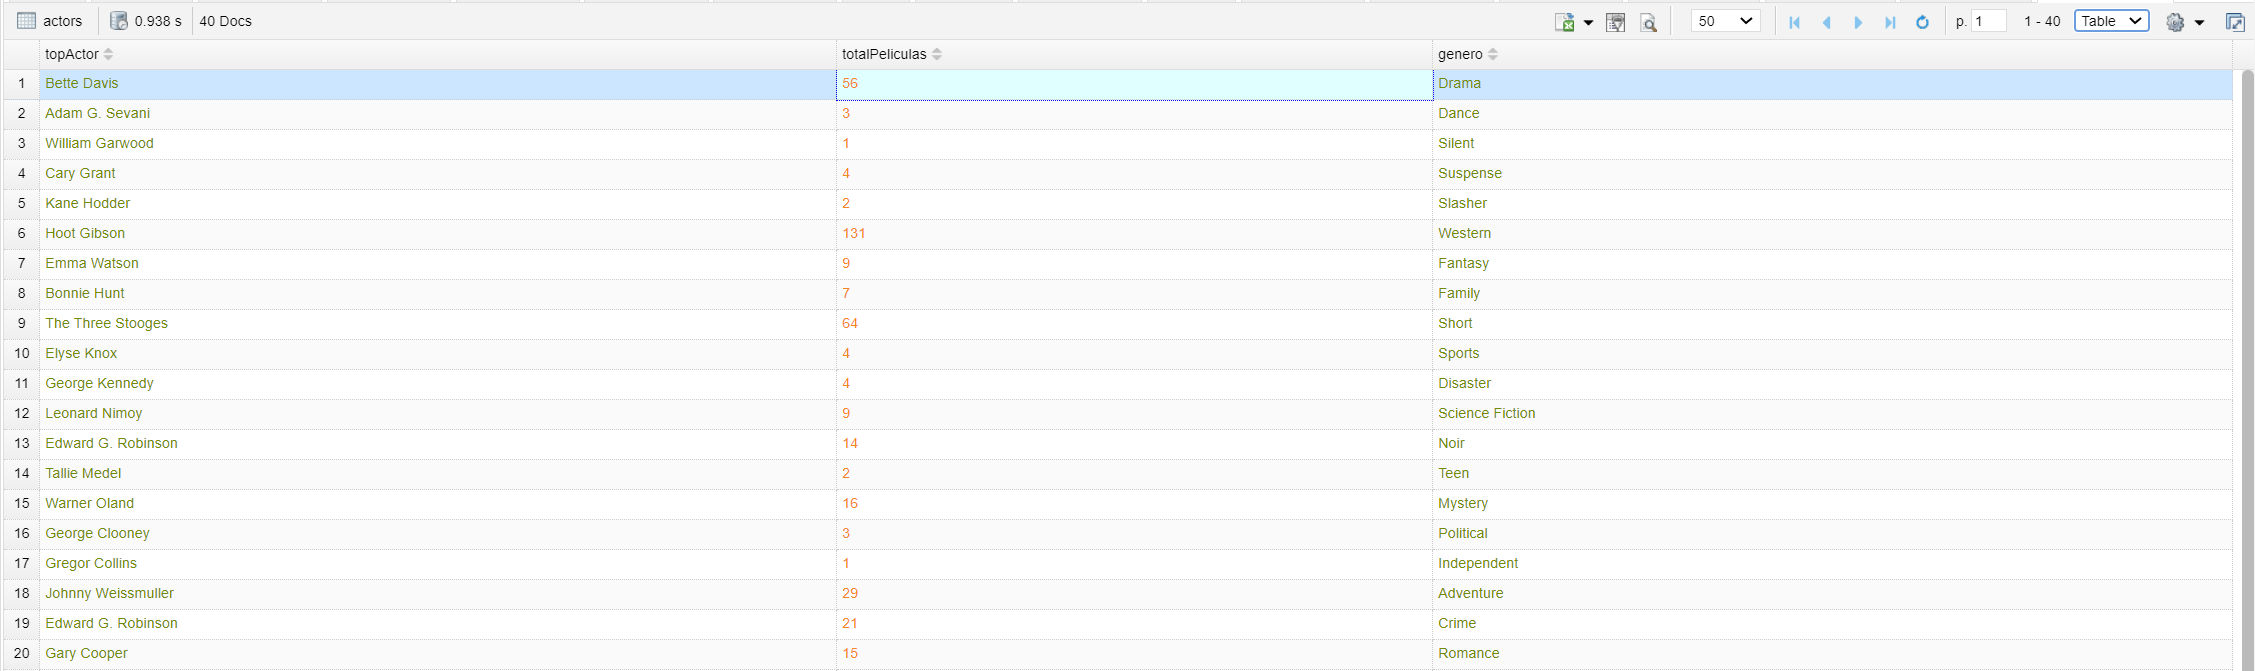
\includegraphics[width=\textwidth]{querys/25_result1.png}
    \end{figure}
    \begin{figure}[H]
            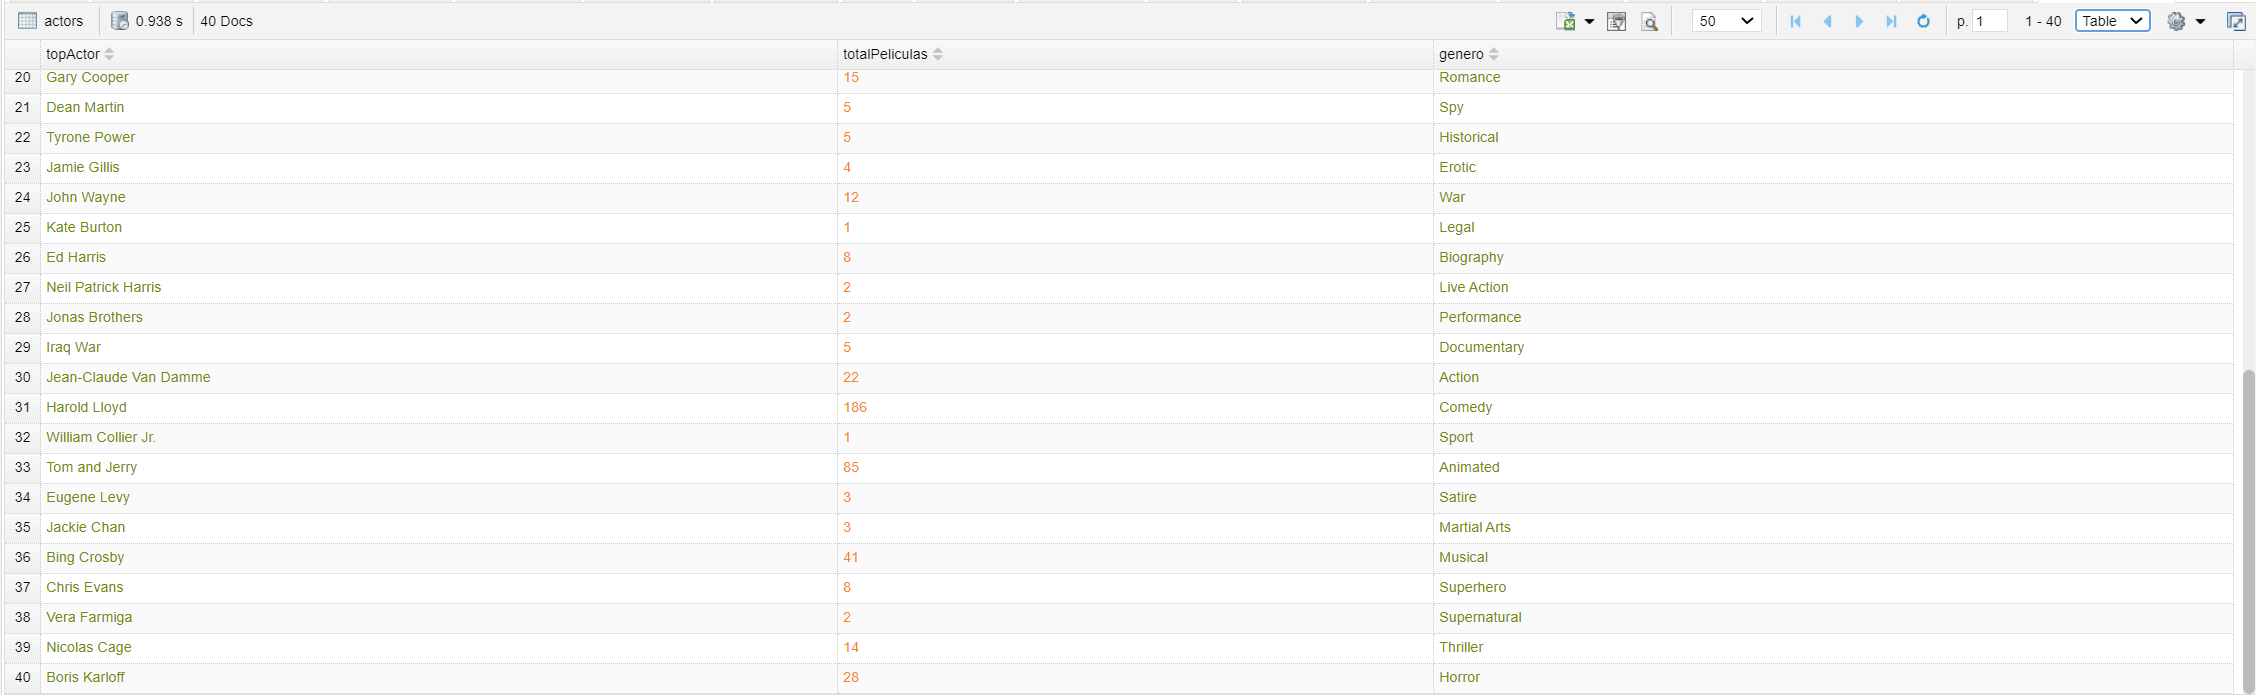
\includegraphics[width=\textwidth]{querys/25_result2.png}
    \end{figure}
    \item \textbf{Ejercicio libre. Sobre \underline{genres}, mostrar el génenro más popular en cada década, mostrando su nombre y el total de películas}. 
    Primero, se exluyen los géneros Undefined. Se usa el addFields para añadir un campo con la década, que se calcula restando al año de la película el resultado de hacer el módulo
    (con \texttt{\$mod}) 10 del año (es decir, restamos las unidades de los años, para quedarnos con las decenas). Se agrupa por década y género y se procede de forma similar al anterior:
    se calcula el total, se ordena por década y total, se agrupa por década para obtener el primer género, y luego se ordena el resultado por década de forma ascendente.
    \begin{figure}[H]
        \begin{subfigure}[b]{0.6\textwidth}
            \centering
            \adjustbox{valign=m}{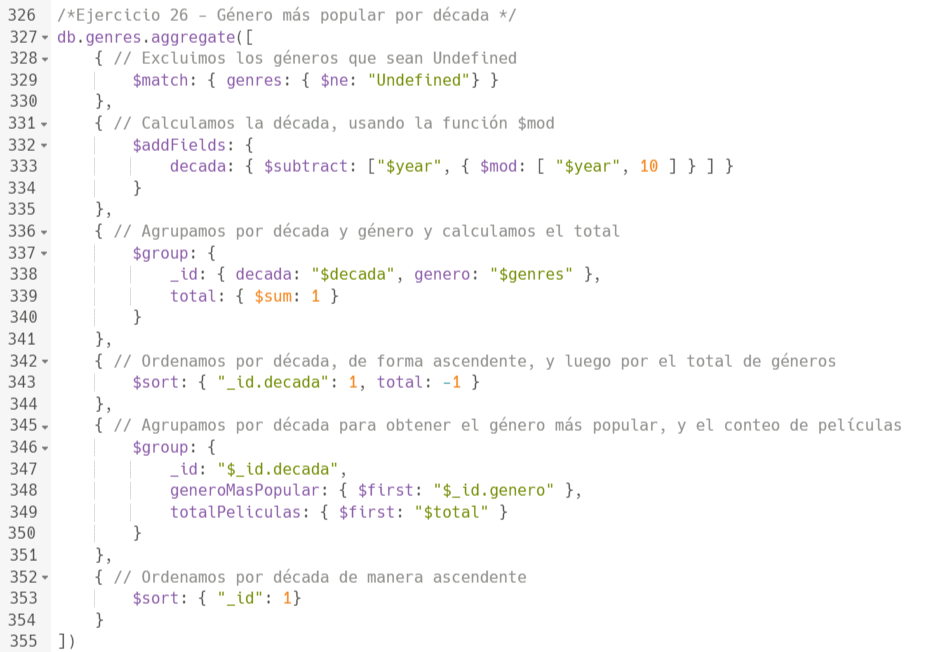
\includegraphics[width=\textwidth]{querys/26_query.png}}
        \end{subfigure}
        \hfill
        \begin{subfigure}[b]{0.4\textwidth}
            \adjustbox{valign=m}{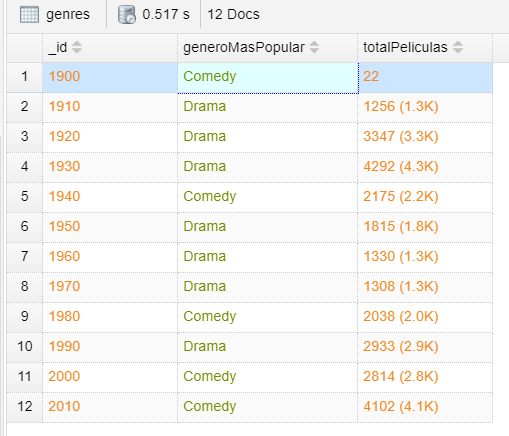
\includegraphics[width=\textwidth]{querys/26_result_tabla.png}}
        \end{subfigure}
   \end{figure}
\end{enumerate}

\end{sloppypar}

\section{Querys de los ejercicios}
\lstinputlisting{querys/querys_noSQL.js}
\end{document}
